\chapter{Week 3: 6\textsuperscript{th}  - 12\textsuperscript{th} Oct}
 \tocless\section{Objectives}
\begin{itemize}
	\item Begin Modelling
	\item Begin I\textsuperscript{2}C communication with the 9DOF
\end{itemize}

%\section{Autonomous Navigation for Flying Robots}
%All ESCs can be connected to the same I$^2$C bus.

 \tocless\section{Modelling}
To create an accurate model for the control of the quad-rotor physical measurements of the quad-rotor had to be carried out. The that have to be measured are as follows the motor gain and time constants $(K_f  ~\mathrm{and} \tau)$ , the inertia of the three axes ($J_{\theta},J_{\phi}~ \mathrm{J_{\psi}}$). 

To ensure that the model is complete enough for a first pass model one would also need to measure the damping coefficient $\beta$ and the motor drag coefficient $D$. The damping coefficient can be found while doing the moment of inertia tests while the drag can be found from doing step response on the motor and back solving to find $D$ by using the general motor equation.  \footnote{Link to explanation of how brushless DC motor work\url{http://educypedia.karadimov.info/library/ems_ch12_nt.pdf}} \footnote{Link to a control assignment of a brushless DC motor (similar to the assignment done in third year) \url{http://support.ctc-control.com/customer/elearning/younkin/driveMotorEquations.pdf}}
\begin{equation}
	J\ddot{\Theta} = K_f i - \beta \dot{\Theta} - D
	\label{motor eqation}
\end{equation}
If one sets $i$ to zero in \eqref{motor eqation} one can find the drag coefficient ($D$) if the damping factor ($\beta$) is known.
Also the mass of the quad-rotor must be found, this can easily found using a spring balance or strain gauge.

 \tocless\subsection{Motor and ESC Speed Test}
The main focus for this week was to collect data that would allow the creation of a accurate model of the quad-rotor. This meant  that trust and speed data would have to be collected so characteristic curves could created. But during the initial test of all four motors  there was huge a huge difference between motor 4 and the rest of the motor characteristic responses. This meant that all four motor would have to be recalibrated to ensure that each motor would have the same characteristic responses (within margins of error).

The results of the input control signal (\gls{pwm}) vs speed can be seen in figure \ref{fig: PWM Wavelength vs Speed for Axi Motor} (Note the \gls{pwm} used in this project has a period of  20 \si[mode=text]{\milli \second} with a 1-2 \si[mode = text]{\milli \second} pulse duration. Therefore the Duty cycle of the \gls{pwm} signal is 5 - 10 \% ). The graphs that were generated were linear as expected and were plotted in Matlab with a trend line to find the slope of the best fit line for the data sets that were taken for each motor (using ployfit command). This best fix line allows the DC motors to be normalized so that one motor model can be used for the simulation. Note that in order to get a stable aggressive control the motors will have to be reverted back to there accurate model before the code is written in C++ to ensure the best possible control of the quad-rotor.


\begin{figure}[h]
	\centering
	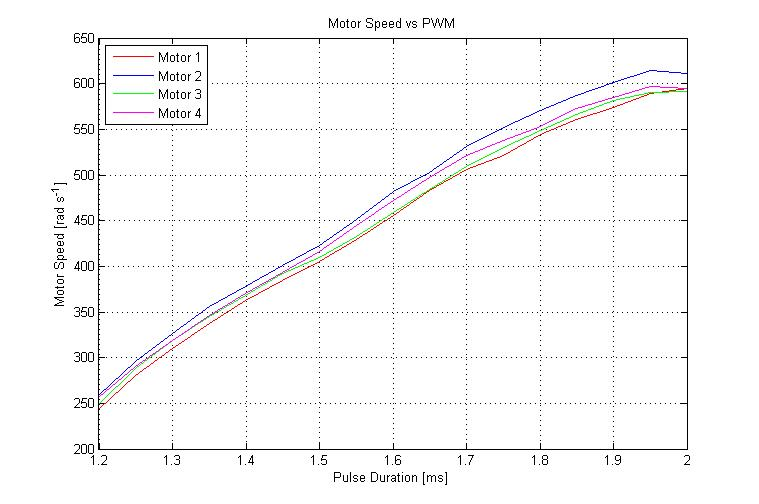
\includegraphics[width=.8\linewidth]{\DocRoot/images/SpeedPWM1}
	\caption{\gls{pwm} pulse duration vs Motor Speed}
	\label{fig: PWM Wavelength vs Speed for Axi Motor}
\end{figure}


 \tocless\subsection{Quad-Copter weight}
The mass of the quad-rotor was acquired using a strain gauge. The mass of the system was found to be 2.26 \si[mode = text]{\kilogram}. Thus the motors will have to supply 22.17  \si[mode = text]{\newton} of thrust to keep the quad-rotor to hovering in the same position. This means that each motor will have to supply at least 5.5425 \si[mode = text]{ \newton} (0.565 \si[mode =text]{\kilogram}) of thrust to keep the quad-rotor a hovering in free space.

 \tocless\subsection{Motor and Propeller Thrust}
The thrust tests were carried out using the strain gauge. The strain gauge gave out mass in \si[mode = text]{\kilogram}'s so the output had to be scaled by gravity (9.81 \si[mode = text]{\meter \per  \square \second}).  The operating point for the quad-rotor was found to be 1.7 \si[mode =text]{\milli \second} as seen in figure \ref{Fig: Motor thrust graph}.  Note this was different to the operating point found by Brendan Barry. Note fro figure \ref{Fig: Motor thrust graph} there is a head room of 10 \si[mode = text ]{\newton}. This means the maximum angle the quad-rotor can go through is 45\textsuperscript{o} so as to allow the quad-rotor some degree of manoeuvrability in 3d space. But if the limit the angle to 20\textsuperscript{o}, the quad-rotor will be capable of lifting 0.8 \si[mode = text]{\kilogram}. 
\begin{figure}[h]
	\centering
	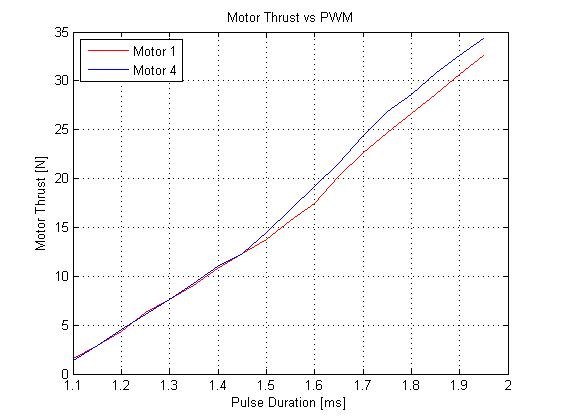
\includegraphics[width=.8\linewidth]{\DocRoot/images/ThrustPWM1}
	\caption{PWM pulse duration vs Motor Thrust}
	\label{Fig: Motor thrust graph}
\end{figure}

 \tocless\section{Communication with 9DOF}
Basic communication with the 9 DOF was accomplished using the i2c\_in (used to write to the device) and  i2c\_out (used to read from the device) during the week. There was problems communicating with the accelerometer as register 2D was entering sleep mode randomly after a revision to the code was made. The register would go from 0x08 (measurement mode) to 0x00 (wakeup mode) and the x-axis, y-axis and z-axis would then read back 0,0,0 respectfully. This problem has be insulated and hopefully code for reading the 9DOF will be in the following week.
%Time constant of motor must be found. Use a small DC motor attached to shaft of Axi motor. Apply step input. Measure DC value from motor. Use 63 percent value to find tau.

%Thrust vs PWM wave relationship must be found. Use newton balance to find relationship. Use similar set up to one shown in A2 of Brendan Barry report. Set scales to zero. Apply PWM wave get weight in kg and convert to Newton Thrust. L %inearize the data in Matlab.

%Motor speed vs PWM wave relationship must also be found. Optical Tachometer used to measure speed of rotation in rpm. Convert rpm to rad/s. Add a second order trend line to find operating point. Linearize at operating point.
%Done

%Inertia tests must be carried out for the frame. The roll and pitch axis can be presumed to be the same. Yaw is different. Ensure batteries, electronics  and sensors are mounted on the test rig. Otherwise inertia values won't be %correct. Add a substitute mass to the centre for microcontroller and associated electronics. Measure magnitude and frequency of oscillation with a voltage across a pot. Calibrate the pot for maximum angles using spirit level. Measure %using Arduino the voltage across. And convert to degrees. Using equations on page 25 of Brendan Barry report calculate various quantities.


%Drag and Inertia of the motors and drag torque of propellers need to be calculated. Find the no load torque in Figure 5.10 on page 26. Add weights to lever at end of shaft until internal resistance overcome. 

%Motor constant of Axi motor given in datasheet. Can be tested for to confirm. 

%Use current transformer to measure currents at different operating speeds.

%Find the operating point. Find weight of quad. Operating point is here for hover. So divide by 4 to spread thrust required evenly over 4 motors.

%Use this to find operating point of PWM wave in secs and speed in rad/s and current in amps.

%Where does the force to angular acceleration constant come from in Simulink diagram

%Magnetic Declination is -17$^{\circ}$ 22' West